\chapter{Work Plan}
\label{chap:WorkPlan}

The execution of this dissertation followed a structured 12-month plan, commencing in November 2024 and culminating in the submission in October 2025. This chapter outlines the strategic phasing of the project, designed to ensure a logical progression from foundational research to final implementation and evaluation.

The timeline was organized into five distinct but overlapping phases, each with specific objectives and deliverables. This approach facilitated agile adaptation while maintaining a clear focus on the project's long-term goals. The complete project schedule, including granular tasks and their dependencies, is visualized in the Gantt chart presented in Figure~\ref{fig:gantt_chart_detailed}.

\begin{figure}[htbp]
    \centering
    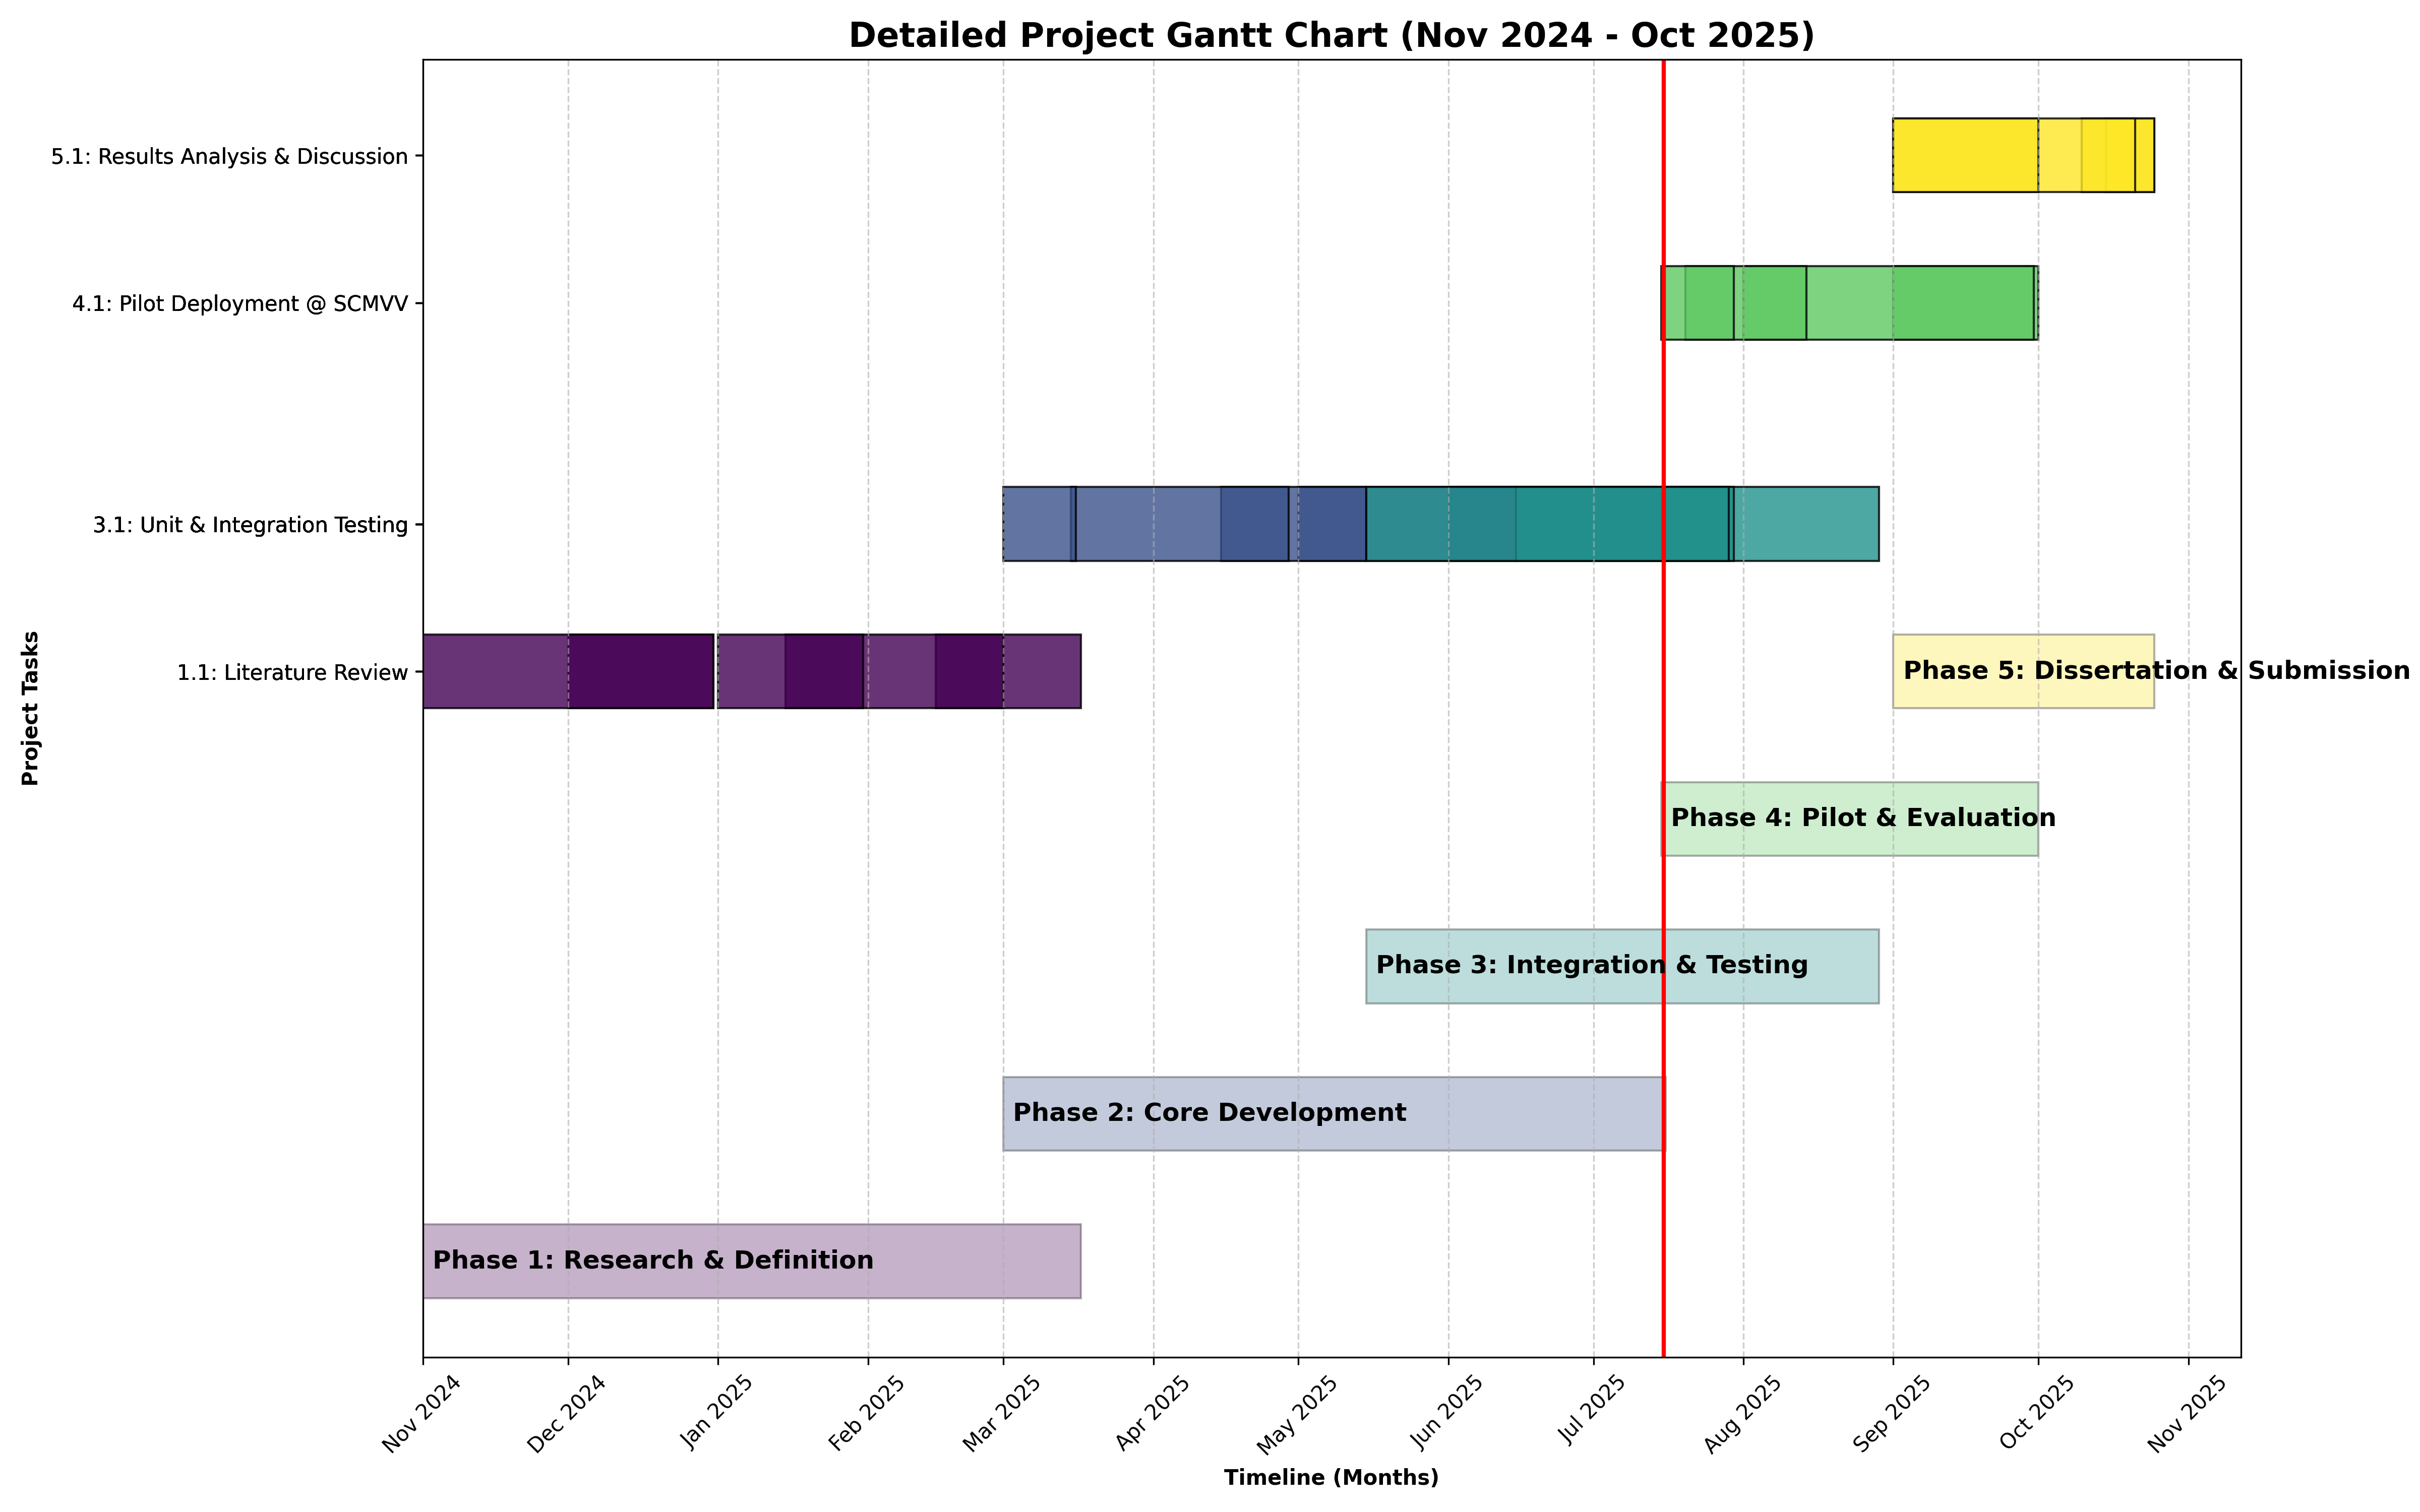
\includegraphics[width=\textwidth]{images/generated/gantt_chart_detailed.png}
    \caption{Detailed Gantt chart illustrating the 12-month project timeline, key phases, and task dependencies from November 2024 to October 2025.}
    \label{fig:gantt_chart_detailed}
\end{figure}

The initial phase, \textit{Research and Definition}, focused on establishing a solid theoretical and empirical foundation through an exhaustive literature review and an in-depth analysis of the existing clinical workflows at SCMVV. This was followed by the \textit{Core Development} phase, where the system's foundational components, including the database, security modules, and core backend logic, were implemented.

Subsequently, the \textit{Integration and Testing} phase ensured that the newly developed modules operated cohesively and could be reliably connected to existing external and legacy systems. The fourth phase, \textit{Pilot and Evaluation}, marked the transition from a development environment to a live clinical setting, where the system was deployed and rigorously evaluated based on user feedback and performance data.

The final phase, \textit{Dissertation and Submission}, was dedicated to the analysis of the collected data, the synthesis of the research findings, and the writing of this dissertation, culminating in its final submission and defense. The detailed methodological framework underpinning the execution of this plan is elaborated upon in the following chapter.

\section{Risk Analysis and Mitigation Strategies}
\label{sec:RiskAnalysis}

A proactive approach to risk management is essential for the successful execution of this project. The risk management plan addresses four key domains: technological, project management, user adoption, and data governance.

The primary technological risk involves integration challenges with the hospital's legacy systems, particularly AIDA-PCE. To mitigate this, a dedicated integration layer will be developed, acting as an anti-corruption shield that isolates the new system from the old. A secondary technical risk pertains to system performance under high load, which will be addressed through continuous load testing and query optimization throughout the development cycle.

In project management, scope creep represents a significant threat. This will be managed through a strict change control process and bi-weekly sprint reviews with stakeholders to ensure alignment with core objectives. Potential delays are mitigated by the modular design, allowing for parallel work streams, and by building buffer time into the project schedule.

A critical sociotechnical risk is the potential for resistance to change from clinical staff. The mitigation strategy is centered on the user-centered co-design approach mentioned in the methodology, ensuring continuous user involvement. This is complemented by a comprehensive training program and the empowerment of clinical champions within each department to drive adoption and provide peer support.

Finally, to address data governance and security risks, compliance with GDPR and robust data protection are paramount. All patient data will be encrypted both at rest and in transit. Access controls will be role-based and strictly enforced, and the system will undergo regular security audits and penetration testing to identify and address vulnerabilities proactively. 